\appendix

\chapter{Model Comparison - Final Topographies}

\begin{figure}[!ht]
	\makebox[\textwidth][c]{
	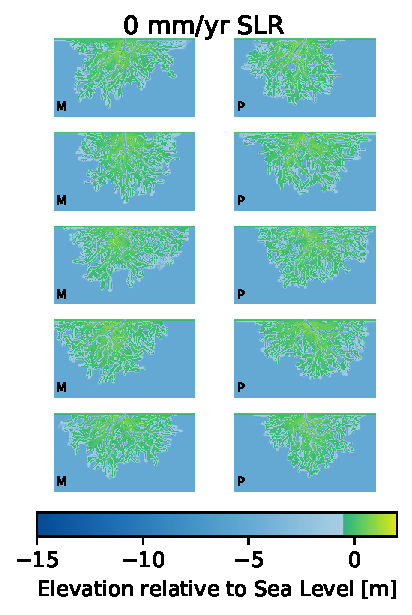
\includegraphics[height=0.95\textheight]{DeltaRCM_ModelComparison/figs/000Topo.pdf}
	}
	\caption{Final topographies for 0 mm/yr replicates. Domain has been clipped.}
	\label{fig:000topo}
\end{figure}

\begin{figure}[!ht]
	\makebox[\textwidth][c]{
	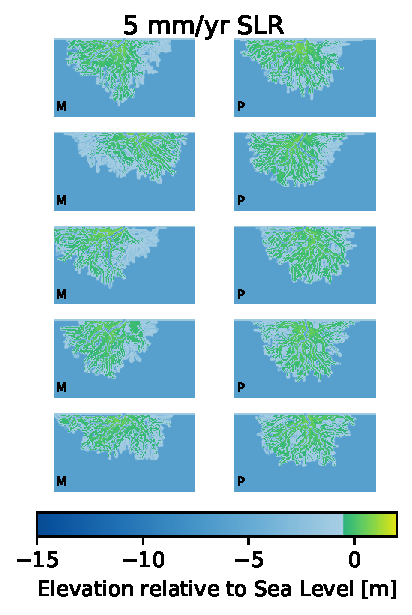
\includegraphics[height=0.95\textheight]{DeltaRCM_ModelComparison/figs/005Topo.pdf}
	}
	\caption{Final topographies for 5 mm/yr replicates. Domain has been clipped.}
	\label{fig:005topo}
\end{figure}

\begin{figure}[!ht]
	\makebox[\textwidth][c]{
	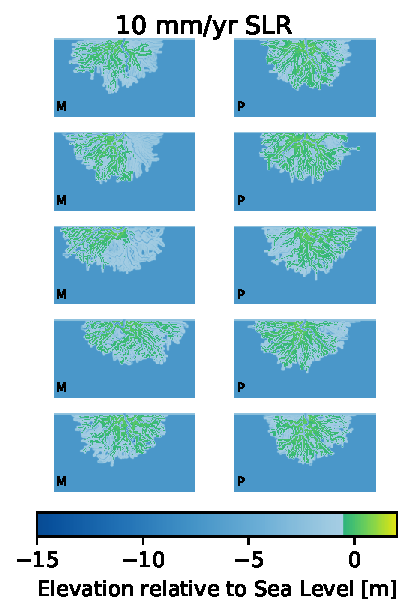
\includegraphics[height=0.95\textheight]{DeltaRCM_ModelComparison/figs/010Topo.pdf}
	}
	\caption{Final topographies for 10 mm/yr replicates. Domain has been clipped.}
	\label{fig:010topo}
\end{figure}

\begin{figure}[!ht]
	\makebox[\textwidth][c]{
	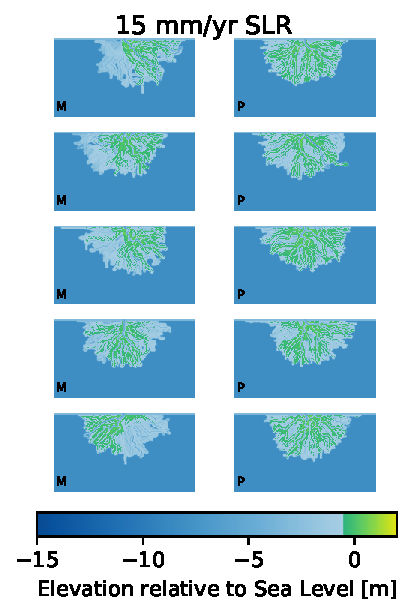
\includegraphics[height=0.95\textheight]{DeltaRCM_ModelComparison/figs/015Topo.pdf}
	}
	\caption{Final topographies for 15 mm/yr replicates. Domain has been clipped.}
	\label{fig:015topo}
\end{figure}

\begin{figure}[!ht]
	\makebox[\textwidth][c]{
	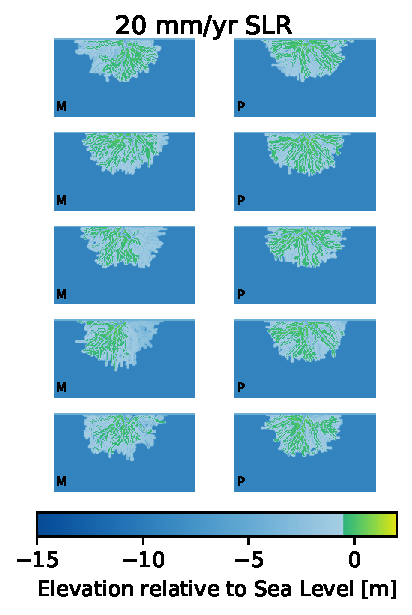
\includegraphics[height=0.95\textheight]{DeltaRCM_ModelComparison/figs/020Topo.pdf}
	}
	\caption{Final topographies for 20 mm/yr replicates. Domain has been clipped.}
	\label{fig:020topo}
\end{figure}

\begin{figure}[!ht]
	\makebox[\textwidth][c]{
	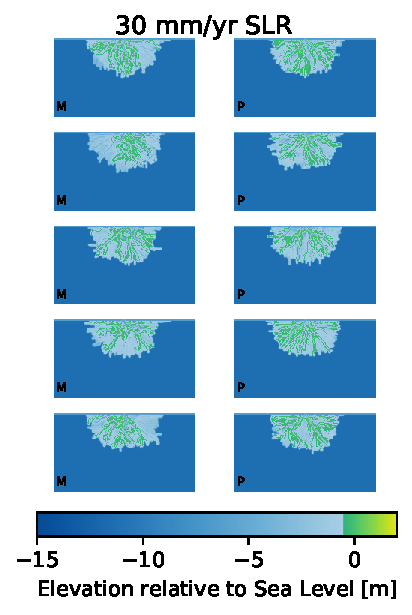
\includegraphics[height=0.95\textheight]{DeltaRCM_ModelComparison/figs/030Topo.pdf}
	}
	\caption{Final topographies for 30 mm/yr replicates. Domain has been clipped.}
	\label{fig:030topo}
\end{figure}

\begin{figure}[!ht]
	\makebox[\textwidth][c]{
	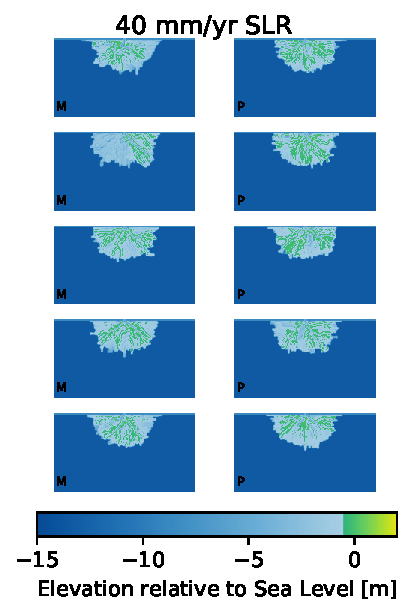
\includegraphics[height=0.95\textheight]{DeltaRCM_ModelComparison/figs/040Topo.pdf}
	}
	\caption{Final topographies for 40 mm/yr replicates. Domain has been clipped.}
	\label{fig:040topo}
\end{figure}